\documentclass[12pt,addpoints,answers]{evalua}
\grado{1$^\circ$ de Secundaria}
\cicloescolar{2023-2024}
\materia{Matemáticas 1}
\unidad{1 y 2}
\title{Examen de la Unidad}
\aprendizajes{
    \item Determina y usa la jerarquía de operaciones y los paréntesis en
    operaciones con números naturales, enteros y
    decimales (para multiplicación y división, sólo números
    positivos).
    \item Resuelve problemas de cálculo de porcentajes, de tanto por
    ciento y de la cantidad base.
}
\author{Prof.: Julio César Melchor Pinto}
\begin{document}
\begin{questions}
    % \section*{\ifprintanswers{Operaciones con decimales}\else{}\fi}
    \question[4]{ Realiza las siguientes operaciones de decimales:

        \begin{multicols}{2}
            \begin{parts}
                \ifprintanswers{\large\part \quad \opadd[hfactor=decimal,resultstyle=\color{red},carryadd=true,carrysub=false]{24.97}{19.34} \\[3em]}
                \else{          \large\part \quad \opadd[hfactor=decimal,resultstyle=\color{white},carryadd=false,carrysub=false]{24.97}{19.34} \\[3em]}
                \fi

                \ifprintanswers{\large\part  \quad  \opsub[hfactor=decimal,resultstyle=\color{red},carrysub=true]{968.31}{134.67} \\[1ex]}
                \else{          \large\part  \quad  \opsub[hfactor=decimal,resultstyle=\color{white},carrysub=false]{968.31}{134.67} \\[1ex]}
                \fi
                \columnbreak%

                \ifprintanswers{\part \quad \opmul[hfactor=decimal,resultstyle=\color{red},displayintermediary=all]{198.4}{12.2} \\[4em]}
                \else{          \large\part \quad \opmul[hfactor=decimal,resultstyle=\color{white},displayintermediary=None]{198.4}{12.2} \\[4em]}
                \fi

                \ifprintanswers{\large\part\opdiv[period,style=text,hrulewidth=0.2pt,vruleperiod=0.7,hfactor=decimal,resultstyle=\color{red}]{8.32}{1.2}}
                \else{          \large\part  \quad $1.2 \overline{) \ 8.32 \ }$}
                \fi
            \end{parts}
        \end{multicols}
    }

    % \subsection*{\ifprintanswers{Resolución de problemas}\else{}\fi}

    \question[5] Resuelve los siguientes problemas:
    \begin{parts}
        \part La mamá de Susana compró 11 m (metros) de franela y pagó 103.40 pesos. ¿Cuánto cuesta el metro de franela?

        \begin{solutionbox}{2cm}
            \opdiv[hfactor=decimal,resultstyle={\ifprintanswers{\color{red}}\else{\color{white}}\fi},displayintermediary=None,carryadd=false,carrysub=false]{103.40}{11}
        \end{solutionbox}

        % \part El precio de 385 artículos comerciales es de 1,232 pesos. ¿Cuál es el precio unitario de cada artículo?

        % \begin{solutionbox}{2cm}
        %     \opdiv[hfactor=decimal,resultstyle=\color{white},displayintermediary=None,carryadd=false,carrysub=false]{1232}{385}
        % \end{solutionbox}
    \end{parts}

    \newpage
    % \section*{\ifprintanswers{Operaciones con fracciones}\else{}\fi}

    % \subsection*{\ifprintanswers{Operaciones con fracciones}\else{}\fi}

    \question[4] Realiza las siguientes operaciones con fracciones:

    \begin{multicols}{2}

        \begin{parts}\large
            \part $\dfrac{3}{5}+\dfrac{2}{5}=$ \fillin[$\dfrac{5}{5}=1$][0in] \\[3em]

            \part $ \dfrac{3}{5} \divisionsymbol\dfrac{2}{3}=$ \fillin[$\dfrac{9}{10}$][0in]  \\[1em]

            \columnbreak%

            \part $\dfrac{7}{8}-\dfrac{3}{4}=$ \fillin[$\dfrac{7}{8}-\dfrac{6}{8}=\dfrac{1}{8}$][0in] \\[3em]

            \part $\dfrac{7}{8}\times\dfrac{3}{4}=$ \fillin[$\dfrac{21}{32}$][0in]  \\[1em]

            % \columnbreak%

            % \part $\dfrac{7}{8}+\dfrac{3}{4}=$ \fillin[$\dfrac{7}{8}+\dfrac{6}{8}=\dfrac{13}{8}$][0in]  \\[3em]

            % \part $ \dfrac{7}{8} \divisionsymbol \dfrac{3}{4}=$ \fillin[$\dfrac{28}{24}=\dfrac{14}{12}$][0in]  \\[1em]

        \end{parts}
    \end{multicols}


    % \subsection*{\ifprintanswers{Resolución de problemas}\else{}\fi}

    \question[5] Resuelve los siguientes problemas:

    \begin{parts}
        % \part Un granjero siembra 2/5 de su granja con maíz y 3/10 con soya, ¿qué cantidad de su granja queda por sembrar?

        % \begin{solutionbox}{2.5cm}
        %     Para conocer la cantidad de su granja que queda por sembrar, se debe restar 2/5 y 3/10 a 1; entonces:
        %     \[1-\dfrac{2}{5}-\dfrac{3}{10}=\dfrac{10}{10}-\dfrac{4}{10}-\dfrac{3}{10}=\dfrac{3}{10}\]

        % \end{solutionbox}

        \part Un reloj se adelanta 3/7 de minuto cada hora. ¿Cuánto se adelantará en 5 horas?

        \begin{solutionbox}{2.5cm}
            Para conocer cuánto se adelantará en 5 horas, se debe multiplicar 3/7 por 5; entonces:
            \[\dfrac{3}{7}\times 5=\dfrac{15}{7}\]
        \end{solutionbox}
    \end{parts}

    % \section*{\ifprintanswers{Porcentajes}\else{}\fi}
    % \subsection*{\ifprintanswers{Porcentajes a decimal}\else{}\fi}

    \question[3] Escribe como decimal los siguientes porcentajes:

    \begin{multicols}{3}
        \begin{parts}\large
            \part $10.8\% =$ \fillin[0.108][0in]

            \part $5\% =$ \fillin[0.05][0in]

            \part $0.5\% =$ \fillin[0.005][0in]
        \end{parts}
    \end{multicols}

    % \newpage
    % \subsection*{\ifprintanswers{Decimal a porcentaje}\else{}\fi}

    \question[3] Escribe como porcentaje los siguientes decimales:

    \begin{multicols}{3}
        \begin{parts}\large
            \part $0.704=\quad$  \fillin[70.4][0in] \%

            \part $0.014=\quad$    \fillin[1.4][0in]   \%

            \part $1=\quad$      \fillin[100][0in]  \%
        \end{parts}
    \end{multicols}

    % \subsection*{\ifprintanswers{Porcentaje de cantidades}\else{}\fi}

    \question[6] Calcula el porcentaje de las siguientes cantidades:

    \begin{parts}
        \setlength{\columnsep}{1.2cm}
        \begin{multicols}{3}
            \part  {\large 15\% de 900 es: \fillin[135][0in] }

            \begin{solutionbox}{2cm}
                \[900\times\dfrac{15}{100}=135\]
            \end{solutionbox}

            \part  {\large 0.5\% de 1200 es: \fillin[6][0in] }

            \begin{solutionbox}{2cm}
                \[1200\times\dfrac{0.5}{100}=6\]
            \end{solutionbox}

            \part  {\large 3.5\% de 415 es: \fillin[14.525][0in] }

            \begin{solutionbox}{2cm}
                \[415\times\dfrac{3.5}{100}=14.525\]
            \end{solutionbox}
        \end{multicols}

        \begin{multicols}{2}

            \part Si se sabe que 210 es el 21\% de cierta cantidad, ¿cuál es esta cantidad?

            \begin{solutionbox}{2.8cm}
                Para conocer la cantidad, se debe dividir 210 entre 21; entonces:
                \[100\times\dfrac{210}{21}=1000\]
            \end{solutionbox}

            \part Si se sabe que 120 es el 35\% de cierta cantidad, ¿cuál es esta cantidad?

            \begin{solutionbox}{2.8cm}
                Para conocer la cantidad, se debe dividir 120 entre 35; entonces:
                \[100\times\dfrac{120}{35}=342.86\]
            \end{solutionbox}

        \end{multicols}

    \end{parts}

    % \subsection*{\ifprintanswers{Resolución de problemas}\else{}\fi}

    % \question[8] Resuelve los siguientes problemas:

    % \begin{multicols}{2}
    %     \begin{parts}
    %         \part El costo de una computadora es de \$12,220 pesos, si la tasa de impuesto es del 15\%. ¿Cuánto será el total a pagar por la computadora?

    %         \begin{solutionbox}{4cm}
    %             Para conocer el total a pagar por la computadora, se debe multiplicar 12220 por 15\%; entonces:
    %             \[12220\times 15\%= 14,050\]
    %             Por lo tanto, el total a pagar por la computadora es de 14053 pesos.
    %         \end{solutionbox}

    %         \part El 24\% de los habitantes de un pueblo tienen menos de 30 años. ¿Cuántos habitantes tiene el pueblo si hay 120 jóvenes menores de 30 años?

    %         \begin{solutionbox}{4cm}
    %             Para conocer el total de habitantes del pueblo, se debe dividir 120 entre 24\%; entonces:
    %             \[100\times\dfrac{120}{24}=500\]
    %             Por lo tanto, el pueblo tiene 500 habitantes.
    %         \end{solutionbox}
    %     \end{parts}
    % \end{multicols}

    \newpage
    \section*{\ifprintanswers{Fracciones}\else{}\fi}

    \subsection*{\ifprintanswers{Clasificación de fracciones}\else{}\fi}

    \question[8] Clasifica las siguientes fracciones en propias, impropias o mixtas:
    \begin{multicols}{2}
        \begin{parts}
            \part $\dfrac{5}{6}=$ \fillin[Propia][1in]   \\
            \part $5\dfrac{5}{11}=$ \fillin[Mixta][1in]  \\
            \part $\dfrac{7}{3}=$ \fillin[Impropia][1in] \\
            % \part $\dfrac{3}{4}=$ \fillin[Propia][1in]   \\
            % \part $1\dfrac{2}{3}=$ \fillin[Mixta][1in]   \\
            % \part $\dfrac{7}{5}=$ \fillin[Impropia][1in] \\
            % \part $\dfrac{7}{8}=$ \fillin[Propia][1in] \\
            % \part $3\dfrac{2}{9}=$ \fillin[Mixta][1in]   \\
            \part $\dfrac{3}{2}=$ \fillin[Impropia][1in]   \\
            % \part $4\dfrac{1}{4}=$ \fillin[Mixta][1in] \\
        \end{parts}
    \end{multicols}
    \subsection*{\ifprintanswers{Representación de fracciones}\else{}\fi}
    \question[4] Escribe sobre la línea la fracción que representa cada imagen:
    \begin{multicols}{2}
        \begin{parts}
            \part 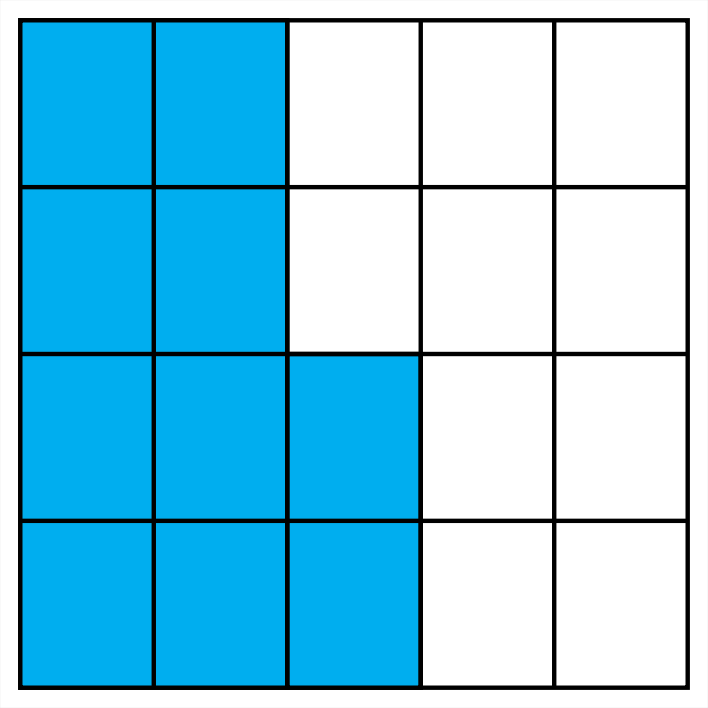
\includegraphics[width=80px]{../images/imagen_frac01.png} \fillin[$\dfrac{10}{20}$][1in]
            \part 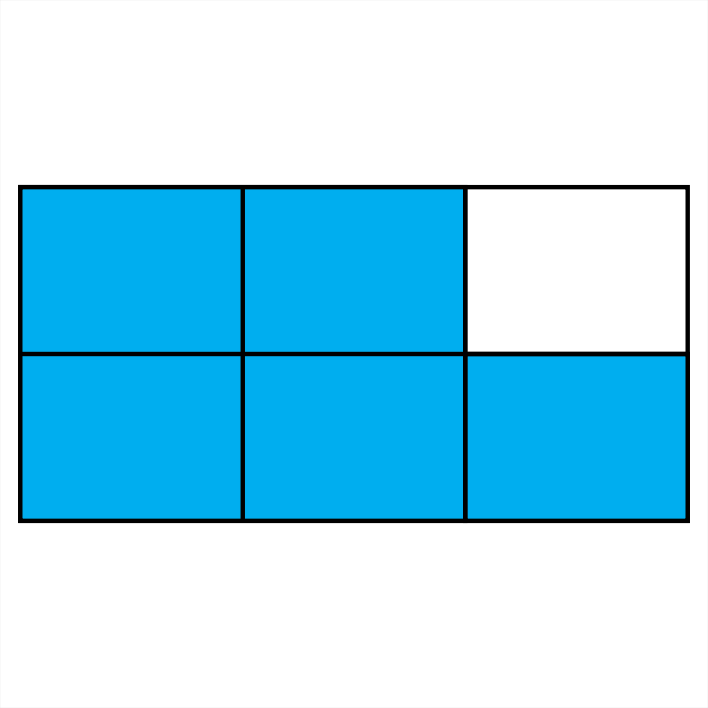
\includegraphics[width=80px]{../images/imagen_frac02.png} \fillin[$\dfrac{5}{6}$][1in]
            % \part 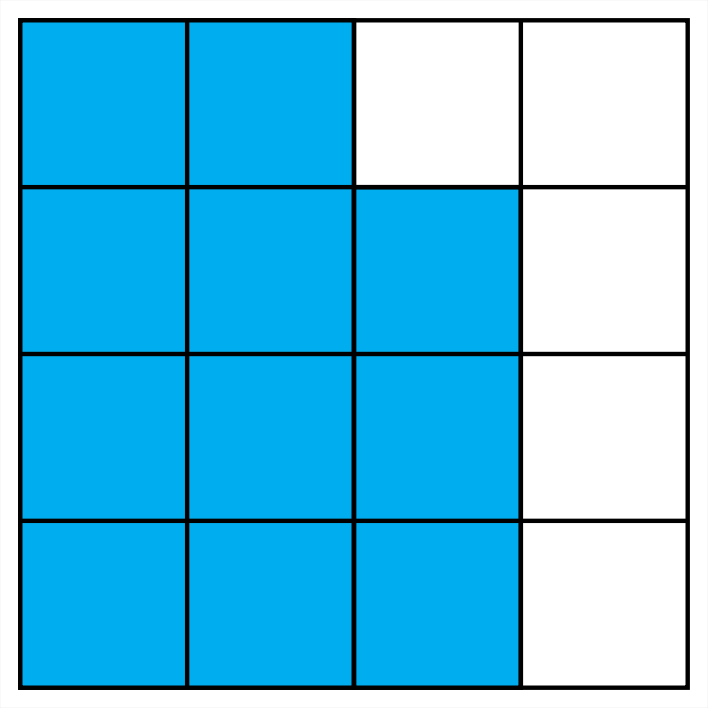
\includegraphics[width=100px]{../images/imagen_frac03.png} \fillin[$\dfrac{10}{20}$][1in]
            % \part 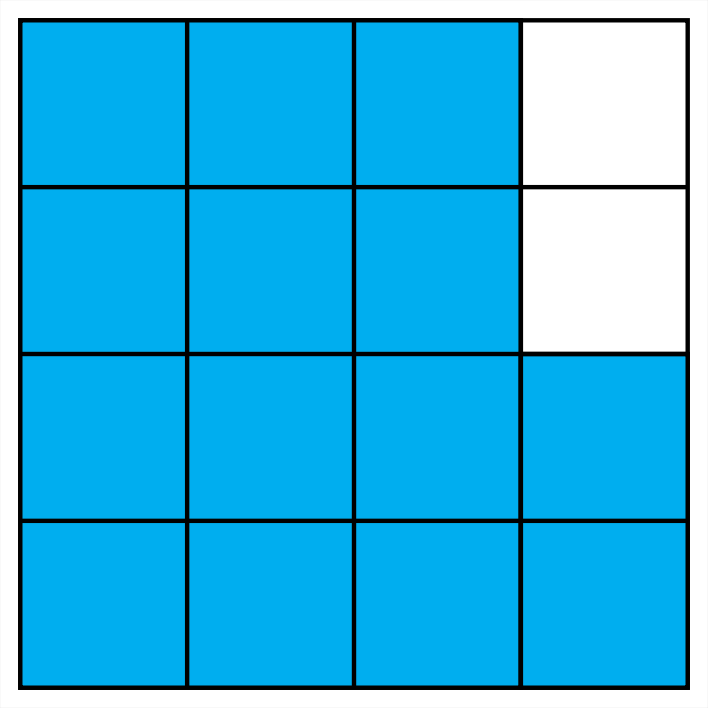
\includegraphics[width=100px]{../images/imagen_frac04.png} \fillin[$\dfrac{10}{20}$][1in]
            % \part 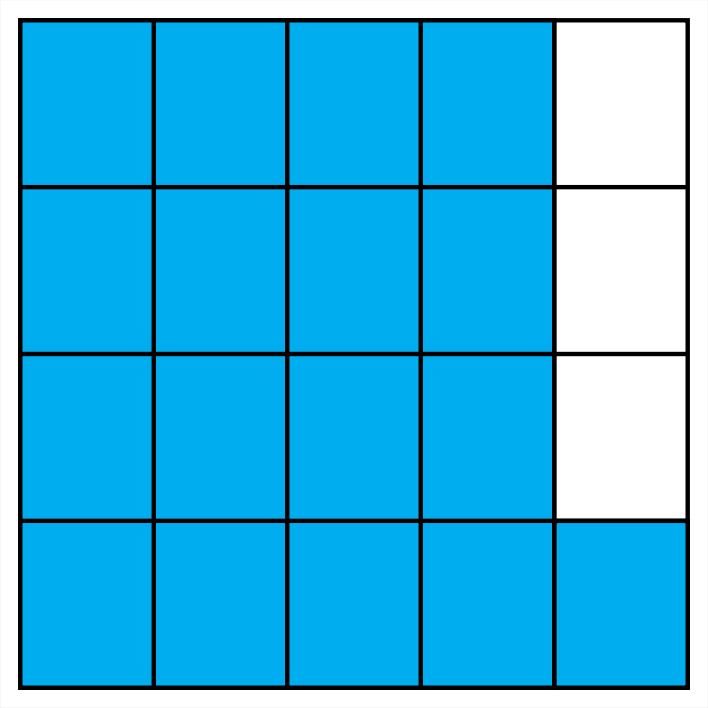
\includegraphics[width=100px]{../images/imagen_frac05.png} \fillin[$\dfrac{10}{20}$][1in]
            % \part 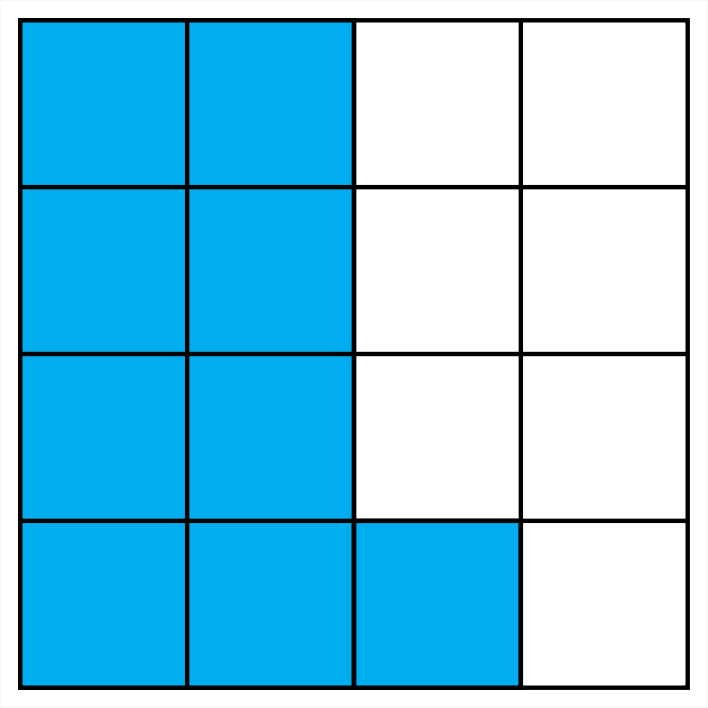
\includegraphics[width=100px]{../images/imagen_frac06.png} \fillin[$\dfrac{10}{20}$][1in]
            % \part 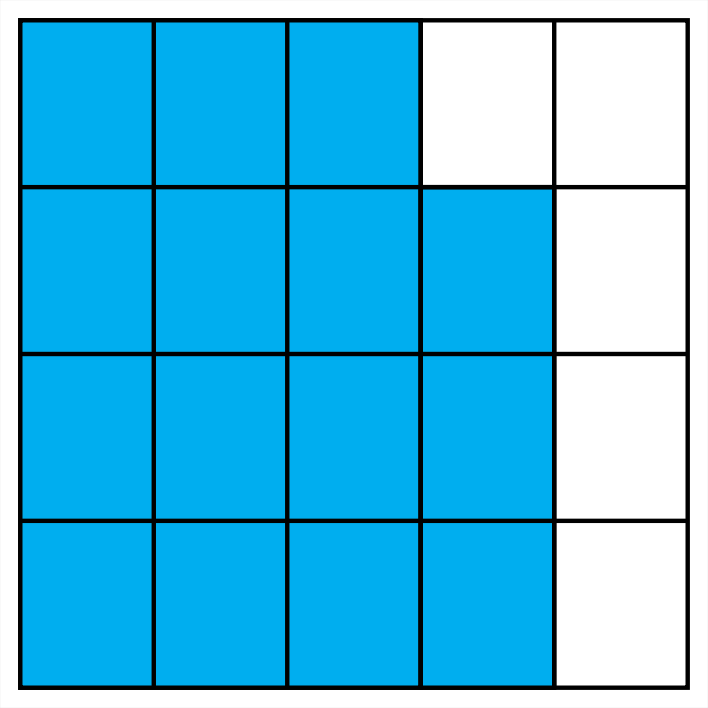
\includegraphics[width=100px]{../images/imagen_frac07.png} \fillin[$\dfrac{10}{20}$][1in]
            % \part 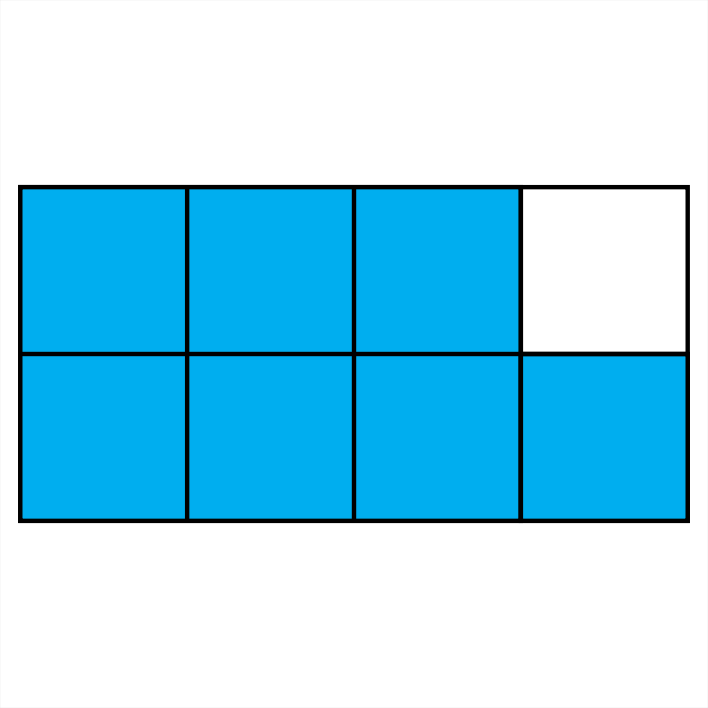
\includegraphics[width=100px]{../images/imagen_frac08.png} \fillin[$\dfrac{10}{20}$][1in]
            % \part 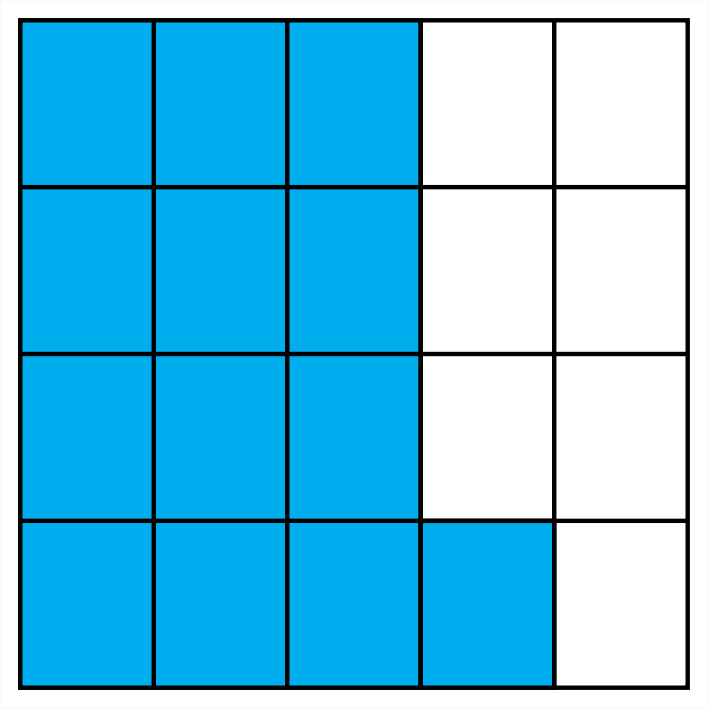
\includegraphics[width=100px]{../images/imagen_frac09.png} \fillin[$\dfrac{10}{20}$][1in]
            % \part 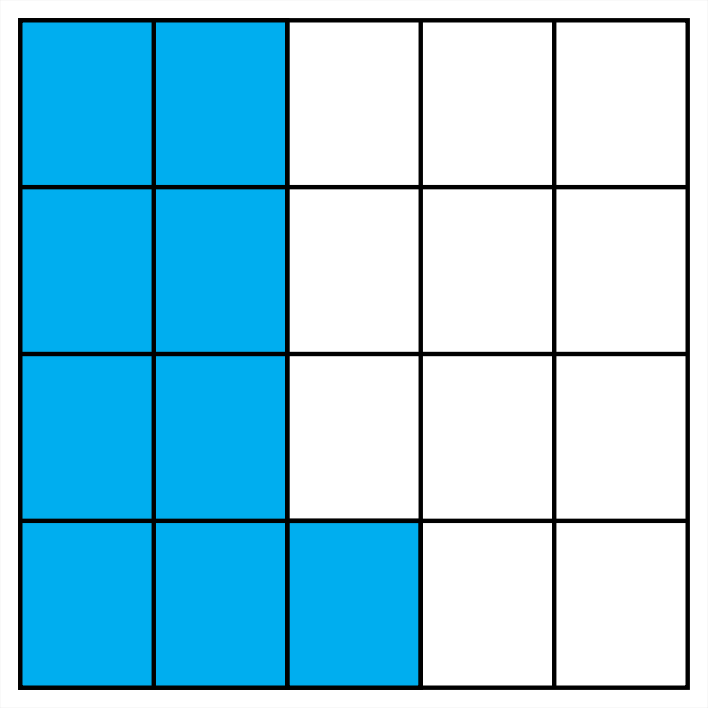
\includegraphics[width=100px]{../images/imagen_frac10.png} \fillin[$\dfrac{10}{20}$][1in]
        \end{parts}
    \end{multicols}

    \subsection*{\ifprintanswers{Nombre de fracciones}\else{}\fi}

    \question[4] Escribe la fracción que corresponda en cada inciso:
    \begin{parts}
        % \part ¿Cómo se escribe numéricamente la fracción \textbf{ocho quintos}?    \fillin[$\dfrac{8}{5}$][0in]  \\
        \part ¿Cómo se escribe numéricamente la fracción \textbf{seis onceavos}?   \fillin[$\dfrac{6}{11}$][0in] \\
        % \part ¿Cómo se escribe numéricamente la fracción \textbf{dos séptimos}?    \fillin[$\dfrac{2}{7}$][0in]  \\
        \part ¿Cómo se escribe numéricamente la fracción \textbf{once medios}?     \fillin[$\dfrac{11}{2}$][0in] \\
        % \part ¿Cómo se escribe numéricamente la fracción \textbf{diez décimos}?    \fillin[$\dfrac{10}{10}$][0in]\\
    \end{parts}

    \subsection*{\ifprintanswers{Fracciones en la recta numérica}\else{}\fi}

    \question[4] Escribe la fracción que representa el punto en la recta numérica
    \begin{multicols}{2}
        \begin{parts}
            \part 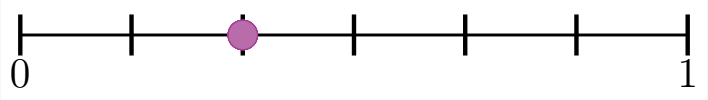
\includegraphics[width=150px]{../images/recta_num_frac01.png} \\[-0.5em] \fillin[$\dfrac{2}{6}$][2in]
            \part 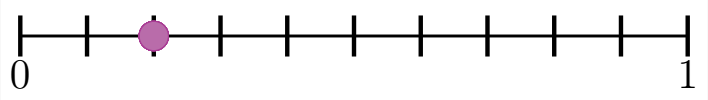
\includegraphics[width=150px]{../images/recta_num_frac02.png} \\[-0.5em] \fillin[$\dfrac{2}{10}$][2in]
            % \part 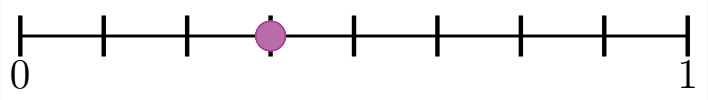
\includegraphics[width=150px]{../images/recta_num_frac03.png} \\[-0.5em] \fillin[$\dfrac{2}{6}$][1.5in]
            % \part 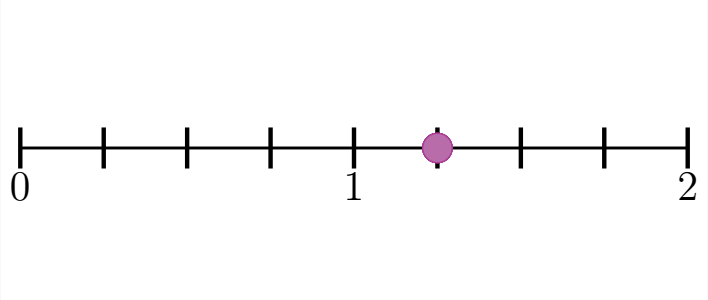
\includegraphics[width=150px]{../images/recta_num_frac04.png} \\[-0.5em] \fillin[$\dfrac{2}{6}$][1.5in]
            % \part 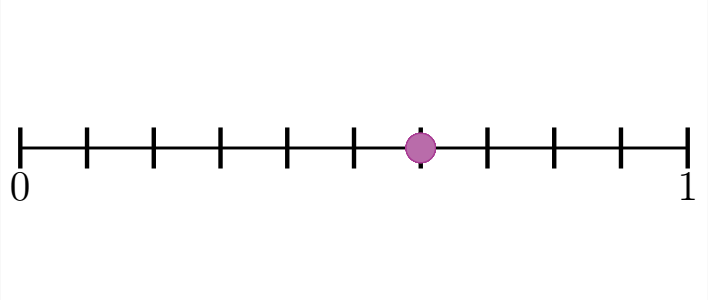
\includegraphics[width=150px]{../images/recta_num_frac05.png} \\[-0.5em] \fillin[$\dfrac{2}{6}$][1.5in]
            % \part 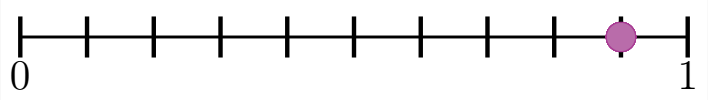
\includegraphics[width=150px]{../images/recta_num_frac06.png} \\[-0.5em] \fillin[$\dfrac{2}{6}$][1.5in]
            % \part 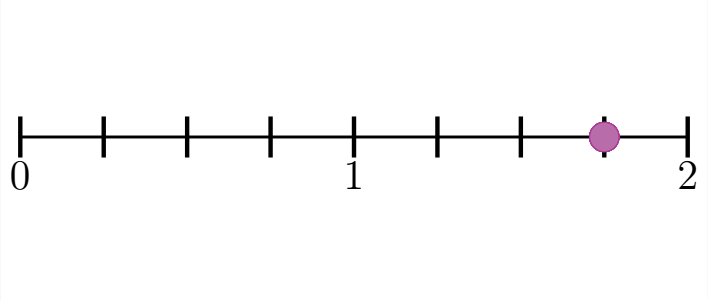
\includegraphics[width=150px]{../images/recta_num_frac07.png} \\[-0.5em] \fillin[$\dfrac{2}{6}$][1.5in]
            % \part 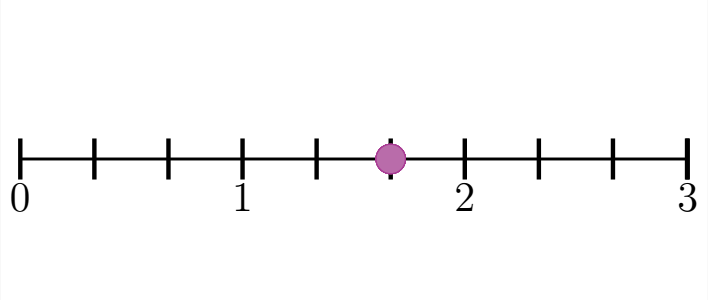
\includegraphics[width=150px]{../images/recta_num_frac08.png} \\[-0.5em] \fillin[$\dfrac{2}{6}$][1.5in]
            % \part 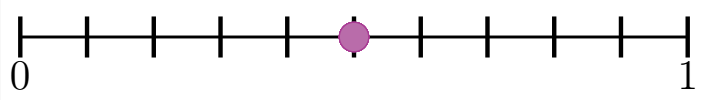
\includegraphics[width=150px]{../images/recta_num_frac09.png} \\[-0.5em] \fillin[$\dfrac{2}{6}$][1.5in]
            % \part 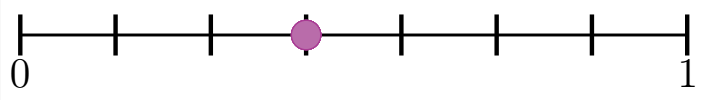
\includegraphics[width=150px]{../images/recta_num_frac10.png} \\[-0.5em] \fillin[$\dfrac{2}{6}$][1.5in]
        \end{parts}
    \end{multicols}

    \subsection*{\ifprintanswers{Conversión de fracciones}\else{}\fi}

    \question[4] Convierte la siguientes fracciones impropias a mixtas:
    \begin{multicols}{3}
        \begin{parts}
            \part $\dfrac{13}{3}= $ \fillin[$4\dfrac{1}{3}$][0in]
            % \part $\dfrac{63}{10}= $ \fillin[$6\dfrac{3}{10}$][0in]
            \part $\dfrac{51}{5}= $ \fillin[$10\dfrac{1}{5}$][0in]
        \end{parts}
    \end{multicols}

    \newpage
    \section*{\ifprintanswers{Fracciones, M.C.M. y M.C.D.}\else{}\fi}

    \subsection*{\ifprintanswers{Comparación de fracciones}\else{}\fi}

    \question[8] Compara las siguientes fracciones usando los signos mayor que (>), menor que (<) o igual (=):
    \begin{multicols}{3}
        \begin{parts}
            \part $\dfrac{4}{3}$ \fillin[$>$][0.5in] $\dfrac{5}{4}$\\[0.75em]
            \part $\dfrac{1}{3}$ \fillin[$=$][0.5in] $\dfrac{3}{9}$\\[0.75em]
            % \part $\dfrac{2}{3}$ \fillin[$<$][0.5in] $\dfrac{3}{2}$\\[0.75em]
            % \part $\dfrac{3}{4}$ \fillin[$>$][0.5in] $\dfrac{2}{3}$\\[0.75em]
            \part $\dfrac{5}{6}$ \fillin[$>$][0.5in] $\dfrac{4}{5}$\\[0.75em]
            \part $\dfrac{1}{3}$ \fillin[$<$][0.5in] $\dfrac{2}{5}$\\[0.75em]
        \end{parts}
    \end{multicols}

    \subsection*{\ifprintanswers{Fracciones equivalentes}\else{}\fi}
    \question[8] Indica si las siguientes fracciones son equivalentes o no:
    \begin{multicols}{2}
        \begin{parts}
            \part $\dfrac{4}{5}=\dfrac{8}{10}$\qquad
            \begin{oneparcheckboxes}
                \CorrectChoice Sí
                \choice No
            \end{oneparcheckboxes}

            \part $\dfrac{1}{8}=\dfrac{4}{16}$\qquad
            \begin{oneparcheckboxes}
                \choice Sí
                \CorrectChoice No
            \end{oneparcheckboxes}

            \part $\dfrac{1}{5}=\dfrac{5}{10}$\qquad
            \begin{oneparcheckboxes}
                \choice Sí
                \CorrectChoice No
            \end{oneparcheckboxes}

            \part $\dfrac{1}{10}=\dfrac{3}{30}$\qquad
            \begin{oneparcheckboxes}
                \CorrectChoice Sí
                \choice No
            \end{oneparcheckboxes}
        \end{parts}
    \end{multicols}

    \subsection*{\ifprintanswers{M.C.D y M.C.M}\else{}\fi}
    \question[4] Calcula lo que se te pide en cada inciso:
    \begin{parts}
        \part Encuentra el máximo común divisor de 33 y 121. \fillin[$\text{mcd}(33,121)=11$][0in]
        \part Encuentra el mínimo común múltiplo de 2, 3 y 4. \fillin[$\text{mcm}(2,3,4)=12$][0in]
    \end{parts}

    \subsection*{\ifprintanswers{Simplificación de fracciones}\else{}\fi}
    \question[4] Simplifica a su mínima expresión la siguiente fracción usando el máximo común divisor
    \begin{multicols}{2}
        \begin{parts}
            \part $\dfrac{8}{64}=$ \fillin[$\dfrac{1}{8}$][0in]
            \part $\dfrac{6}{42}=$ \fillin[$\dfrac{1}{7}$][0in]
        \end{parts}
    \end{multicols}

    % \subsection*{\ifprintanswers{Resolución de problemas}\else{}\fi}

    % \question[6] María y Jorge tienen 45 bolas blancas, 15 bolas azules y 90 bolas rojas y quieren hacer el mayor número de collares iguales sin que sobre ninguna bola. ¿Cuántos collares iguales pueden hacer?
    % \begin{solutionbox}{4cm}
    %     Se calcula el M.C.D.$(45,15,90) = 15$.\\
    %     Por lo tanto, se pueden hacer 15 collares.
    % \end{solutionbox}
    % \newpage
    % \section*{\ifprintanswers{Números decimales}\else{}\fi}

    \subsection*{\ifprintanswers{Ubicación en la recta numérica}\else{}\fi}

    \question[4] Escribe el número que representa el punto indicado en la recta numérica de cada uno de los siguientes incisos.

    \begin{multicols}{2}
        \begin{parts}
            \part 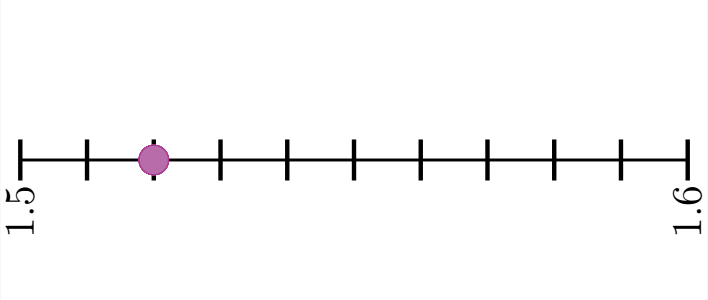
\includegraphics[width=150px]{../images/recta_num_1.52.png} \\[-0.5em] \fillin[$1.52$][1.5in]
            \part 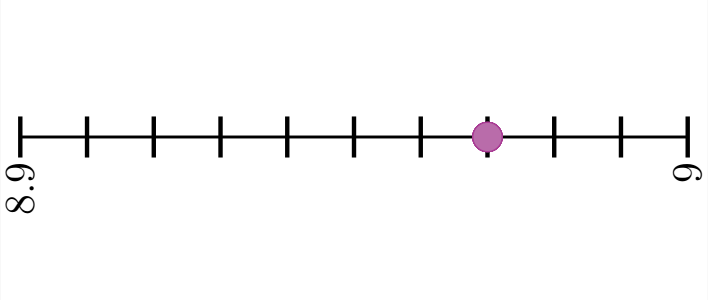
\includegraphics[width=150px]{../images/recta_num_8.97.png} \\[-0.5em]  \fillin[$8.97$][1.5in]  \\[-1.4em]
        \end{parts}
    \end{multicols}

    \subsection*{\ifprintanswers{Porcentajes a decimal}\else{}\fi}

    \question[4] Escribe el número decimal que representa cada porcentaje:

    \begin{multicols}{2}
        \begin{parts}
            \part Convierte 22.9\% a un número decimal. \fillin[$0.229$][0in]
            \part Convierte 6.2\% a un número decimal. \fillin[$0.062$][0in]
        \end{parts}
    \end{multicols}

    \subsection*{\ifprintanswers{Operaciones con múltiplos de 10}\else{}\fi}

    \question[2] Realiza las siguientes operaciones con múltiplos de 10:

    \begin{multicols}{2}
        \begin{parts}
            \part $56.9 \times 100=$ \fillin[$5690$][0in]
            \part $0.712 \times 1000=$ \fillin[$712$][0in]
        \end{parts}
    \end{multicols}


    \subsection*{\ifprintanswers{Conversión de fracciones a decimales}\else{}\fi}
    \question[2] Convierte las siguientes fracciones a decimales:
    \begin{multicols}{2}
        \begin{parts}
            \part $\dfrac{7}{20}=$ \fillin[$0.35$][0in]
            \part $\dfrac{1927}{1000}=$ \fillin[$1.927$][0in]
        \end{parts}
    \end{multicols}

    \subsection*{\ifprintanswers{Conversión de decimales a fracciones}\else{}\fi}
    \question[2] Convierte los siguientes números decimales a una fracción simplificada a su mínima expresión:
    \begin{multicols}{2}
        \begin{parts}
            \part $0.04=$ \fillin[$\dfrac{1}{25}$][0in]
            \part $0.19=$ \fillin[$\dfrac{19}{100}$][0in]
        \end{parts}
    \end{multicols}

    \newpage

    \section*{\ifprintanswers{Números negativos}\else{}\fi}
    \subsection*{\ifprintanswers{Ubicación en la recta numérica}\else{}\fi}
    \question[2] Escribe el número que representa el punto indicado en la recta numérica de cada uno de los siguientes incisos.

    \begin{multicols}{2}
        \begin{parts}
            \part 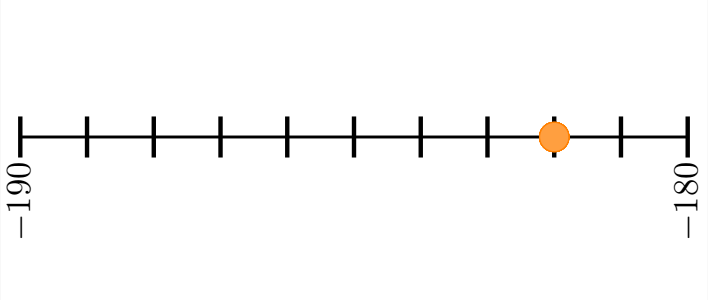
\includegraphics[width=150px]{../images/recta_num_-182.png} \\[-0.5em]   \fillin[$-182$][1.5in]
            \part 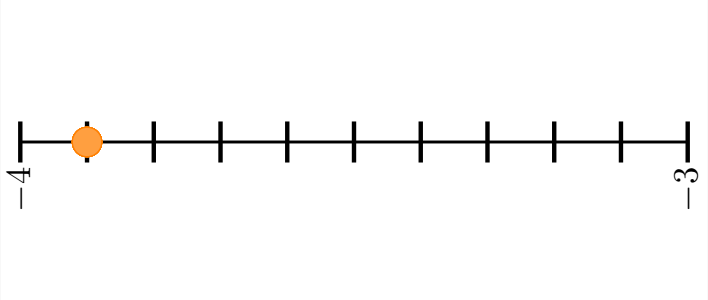
\includegraphics[width=150px]{../images/recta_num_-3.9.png} \\[-0.5em]  \fillin[$-3.9$][1.5in]
        \end{parts}
    \end{multicols}

    \subsection*{\ifprintanswers{Comparación de negativos}\else{}\fi}
    \question[2] Escribe sobre la línea el símbolo de mayor que ($>$), menor que ($<$), o igual ($=$) según corresponda.
    \begin{multicols}{2}
        \begin{parts}
            \part $-182$ \fillin[$>$][0.5in] $-189$\\[0.75em]
            \part $-97$ \fillin[$<$][0.5in] $-96.2$\\[0.75em]
        \end{parts}
    \end{multicols}

    \subsection*{\ifprintanswers{Determina el signo}\else{}\fi}
    \question[2] Determina el signo \textit{positivo} o \textit{negativo} que resulta de las siguientes operaciones:
    \begin{multicols}{2}
        \begin{parts}
            \part $-28-19$ \fillin[Negativo][1in]
            \part $-43+55$ \fillin[Positivo][1in]
        \end{parts}
    \end{multicols}

    \subsection*{\ifprintanswers{Suma y resta con negativos }\else{}\fi}
    \question[2] Realiza las siguientes operaciones con números negativos:
    \begin{multicols}{2}
        \begin{parts}
            \part $-223+67=$ \fillin[$-156$][0in]
            \part $(16)-(-14)$ \fillin[$30$][0in]
        \end{parts}
    \end{multicols}

\end{questions}
\end{document}